
\documentclass [MS] {uclathes}
\usepackage{url}
\usepackage{graphics}
\usepackage[utf8]{inputenc}
\usepackage{amsmath}
\usepackage{hyperref}
\usepackage{graphicx}
\usepackage{subcaption}
\usepackage{mwe}
\usepackage{float}
\DeclareMathOperator{\logit}{logit}


% \input {mymacros}                         % personal LaTeX macros
\hypersetup{
    colorlinks=true,
    linkcolor=blue,
    filecolor=magenta,
    urlcolor=cyan,
    pdftitle={Harrison DiStefano MAS Thesis},
    pdfpagemode=FullScreen
}

%%%%%%%%%%%%%%%%%%%%%%%%%%%%%%%%%%%%%%%%%%%%%%%%%%%%%%%%%%%%%%%%%%%%%%
%
% Usually things live in separate flies.
%
% \input {prelim}                           % preliminary page info

%%%%%%%%%%%%%%%%%%%%%%%%%%%%%%%%%%%%%%%%%%%%%%%%%%%%%%%%%%%%%%%%%%%%%%%%
%                                                                      %
%                          PRELIMINARY PAGES                           %
%                                                                      %
%%%%%%%%%%%%%%%%%%%%%%%%%%%%%%%%%%%%%%%%%%%%%%%%%%%%%%%%%%%%%%%%%%%%%%%%

\title          {TITLE}
\author         {Harrison DiStefano}
\department     {Applied Statistics}
% Note:  degree year should be optional, but as of  5-Feb-96
% it seems required or you get a year of ""2''.   -johnh
\degreeyear     {2022}

%%%%%%%%%%%%%%%%%%%%%%%%%%%%%%%%%%%%%%%%%%%%%%%%%%%%%%%%%%%%%%%%%%%%%%%%

\chair          {Ying Nian Wu}
\member         {Mark S. Handcock}
\member         {Rick Schoenberg}


%%%%%%%%%%%%%%%%%%%%%%%%%%%%%%%%%%%%%%%%%%%%%%%%%%%%%%%%%%%%%%%%%%%%%%%%

%\dedication     {\textsl{To my mother \ldots \\
%                who---among so many other things--- \\
%                saw to it that I learned to touch-type \\
%                while I was still in elementary school}}

%%%%%%%%%%%%%%%%%%%%%%%%%%%%%%%%%%%%%%%%%%%%%%%%%%%%%%%%%%%%%%%%%%%%%%%%



%%%%%%%%%%%%%%%%%%%%%%%%%%%%%%%%%%%%%%%%%%%%%%%%%%%%%%%%%%%%%%%%%%%%%%%%



%%%%%%%%%%%%%%%%%%%%%%%%%%%%%%%%%%%%%%%%%%%%%%%%%%%%%%%%%%%%%%%%%%%%%%%%


%%%%%%%%%%%%%%%%%%%%%%%%%%%%%%%%%%%%%%%%%%%%%%%%%%%%%%%%%%%%%%%%%%%%%%%%

\abstract       {abstract ~350 words recommended}

%%%%%%%%%%%%%%%%%%%%%%%%%%%%%%%%%%%%%%%%%%%%%%%%%%%%%%%%%%%%%%%%%%%%%%%%



\begin {document}
\makeintropages

%%%%%%%%%%%%%%%%%%%%%%%%%%%%%%%%%%%%%%%%%%%%%%%%%%%%%%%%%%%%%%%%%%%%%%
%
% Ordinarily each chapter (at least) is in a separate file.
%
%\input {Intro}                         % Chapter 1 of dissertation
%\input {chapter2}                         % Chapter 2
%\input {chapter3}                         % etc.
%\input {chapter4}
%\input {chapter5}
%\input {chapter6}
%\input {chapter7}
%\input {chapter8}

\chapter{Introduction}




In 


\chapter{Methodology}





\section{LSTM Networks}
 Figure \ref{fig:LSTM_architecture} shows the framework of LSTM.

\begin{figure}[h!]
    \centering
    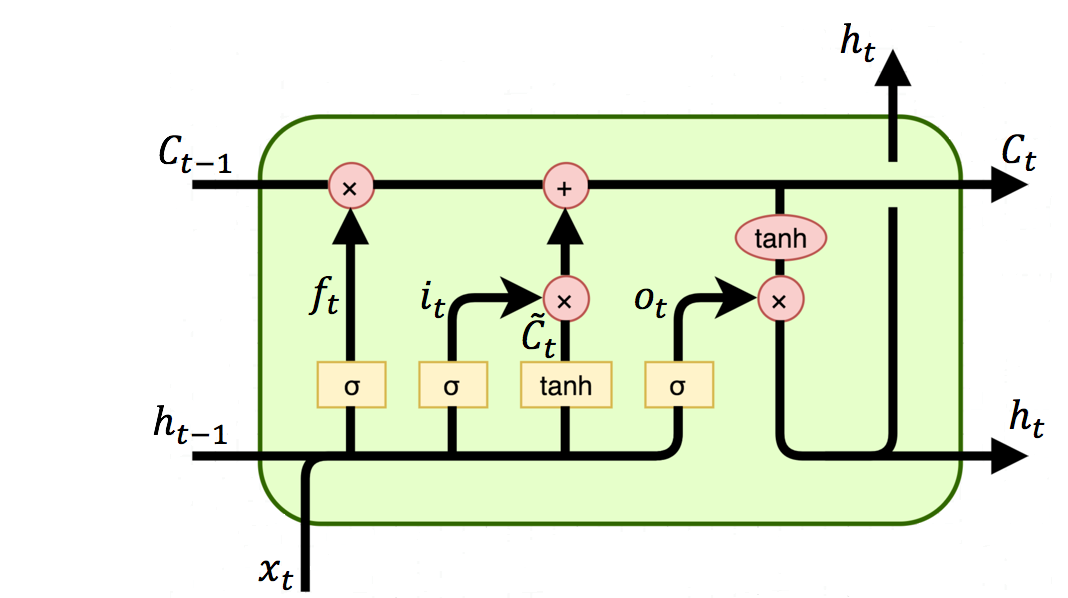
\includegraphics[scale=0.45]{figures/Figure1_frameworkLSTM.png}
    \caption{The framework for LSTM}
    \label{fig:LSTM_architecture}
\end{figure}

The contents of the memory cells $C_t$ are regulated by various gates: 
\begin{itemize}
\item{Forget gate $f_t$}
\item{Input gate $i_t$ }
\item{Output gate $O_t$}
\end{itemize}

The followings are the corresponding formulas.
$$
\begin{aligned}
f_{t} &=\sigma\left(W_{f} \cdot\left[h_{t-1}, x_{t}\right]+b_{f}\right) \\
\tilde{C}_{t} &=\tanh \left(W_{C} \cdot\left[h_{t-1}, x_{t}\right]+b_{C}\right) \\
i_{t} &=\sigma\left(W_{i} \cdot\left[h_{t-1}, x_{t}\right]+b_{i}\right) \\
C_{t} &=f_{t} * C_{t-1}+i_{t} v \tilde{C}_{t} \\
o_{t} &=\sigma\left(W_{o} \cdot\left[h_{t-1}, x_{t}\right]+b_{o}\right) \\
h_{t} &=o_{t} \otimes \tanh \left(C_{t}\right)
\end{aligned}
$$

$W_n$ is the weight matrices of the input and recurrent connections for the input gate, the output gate, the forget gate, or the cell state. $b_n$ is the bias terms for the same components. $\otimes$ is the element-wise product of two vectors. $\sigma$ is a sigmoid function \cite{fager_wil_chew_2019}.


\chapter{Data}
\section{Data Source}
The United States housing price data and supply data used for training and testing is retrieved from the Federal Reserve Bank of St. Louis (FRED), sourced from the relevant official U.S. bureaus \cite{us_census_bureau_median_1963}\cite{us_census_bureau_monthly_1963}. These time series data sets contain 236 quarterly median housing prices in the U.S. from January 1963 until January 2022 and 712 monthly new U.S. housing supply ratios from January 1963 until April 2022. Economic data is taken from Robert Shiller's data set used in his book \textit{Irrational Exuberance}\cite{online_data_robert_shiller} and consists 1,816 rows of monthly economic data from January 1871 until May 2022.

\section{Data Details}

\begin{table}[H]
\centering
\renewcommand{\arraystretch}{0.75}
\caption{Data Attribute Information}
\label{tab:Attribute_Info}
\begin{tabular}{c|r|l} \hline
\textbf{\#}   & \textbf{Label}             & \textbf{Description}                               \\ 
\hline \hline
1  &            DATE                       & First date of the period to which data corresponds, \\
   &                                       & e.g. 01-01-1963 for first fiscal quarter of 1963 if      \\
   &                                       & quarterly data                                   \\
2  &            MSPUS                      & Median U.S. housing prices over the given fiscal \\
   &                                       & quarter in DATE. Target variable for this paper  \\
3  &            MSACSR                     & Monthly supply of new U.S. houses, calculated by \\           
   &                                       & ratio of new houses for sale to new houses sold   \\
4  &            S\&P Comp.                 & Value of S\&P Composite index on the given date \\
5  &            Dividend                   & Total dividends per share of the S\&P Comp. \\
6  &            Earnings                   & Earnings per share of the S\&P Comp. \\
7  &            CPI                        & Weighted average price of basket of consumer goods\\
8  &            Long Interest Rate GS10    & Market yield on U.S. Treasury 10-Year Securities \\
9  &            Real Price                 & Value of S\&P Comp. adjusted for inflation \\
10 &            Real Dividend              & Dividend adjusted for inflation \\
11 &            Real Total Return Price    & Cumulative total return of S\&P Comp. since 1963 \\
12 &            Real Earnings              & Earnings adjusted for inflation \\
13 &            CAPE                       & CAPE ratio of S\&P Comp. \\
14 &            Total Return CAPE          & CAPE with dividends reinvested \\
15 &            Excess CAPE Yield          & Inverse of CAPE ratio \\
16 &            Monthly Total Bond Returns & Shiller Monthly Total Bond Returns \\
17 &            Real Total Bond Returns    & Inflation adjusted Shiller bond returns \\
18 &            10 Year Stock Real Return  & Moving 10 year infl. adjusted S\&P Comp. returns \\
19 &            10 Year Bonds Real Return  & Moving 10 year infl. adjusted Shiller returns \\
20 &            10 Year Excess Returns     & Inverse of 10 year stock real returns \\
\hline
\end{tabular}
\end{table}

The data consists of quarterly median U.S. housing prices, the monthly supply of new U.S. houses, and 17 monthly U.S. macroeconomic statistics for a total of 1816 months from January 1871 until May 2022. However, due to the price data being quarterly and the economic data being monthly, price information is missing from two out of every three months. We will fix this in the Data Cleaning section.





\section{Data Cleaning}

We begin by cleaning the data to prepare it for analysis and modelling. The data comes from several sources and so needs to be massaged into a cohesive unit so that it can be passed easily through our tools. The data also needs to be processed in order to match the assumptions of our models.

As mentioned previously, there are 1816 rows (months) of economic data and 712 of housing price data. Since there are fewer months of pricing data, the target variable, than economic data, we remove all rows with dates falling outside the range of the pricing data leaving 712 rows.

\subsection{Null Values}

Part of massaging our dataset includes handling missing values, either by filling or removing them from the dataset in order to perform analysis. We will do both filling through interpolation and removal of some values columns and rows that are less necessary.

\subsubsection{Interpolation}
The economic data is monthly and the U.S. median house price data is quarterly as shown in Table \ref{tab:Before_Interpolation}

\begin{table}[H]
\centering
\renewcommand{\arraystretch}{0.75}
\caption{Six Months of U.S. Housing Supply and Price Data with Missing Values}
\label{tab:Before_Interpolation}
\begin{tabular}{c|c|c} \hline
\textbf{DATE}   & \textbf{MSACSR}     & \textbf{MSPUS}  \\ 
\hline \hline
1963-01-01      & 4.7                 & 17800.00        \\
1963-02-01      & 6.6                 & NULL            \\
1963-03-01      & 6.4                 & NULL            \\
1963-04-01      & 5.3                 & 18000.00        \\
1963-05-01      & 5.1                 & NULL            \\
1963-06-01      & 6.0                 & NULL            \\
1963-07-01      & 4.6                 & 17900.00        \\
\hline
\end{tabular}
\end{table}

To avoid removing all of these null values and with them two-thirds of the granularity of economic data, we interpolate between the known price values to fill what is missing.

To do this we use linear interpolation, this is done by calculating the equation of the line between two known points and plugging in the x values for the unknown points--here that is the DATE--to get the price that lies on that line. This is done as follows:
$$
\begin{aligned}
y &= \frac{y_{0}\left(x_{1} - x \right) + y_{1}\left(x_{1} - x \right)}{x_{1} - x_{0}} \\
\end{aligned}
$$

Where $\left(x_{0}, y_{0}\right)$ and $\left(x_{1}, y_{1}\right)$ are the coordinates of the two known points, and $y$ is the value along the straight line between those two points at value $x$. \cite{encyclopediaofmath_linear_interpolation} 

\begin{figure}[h!]
    \centering
    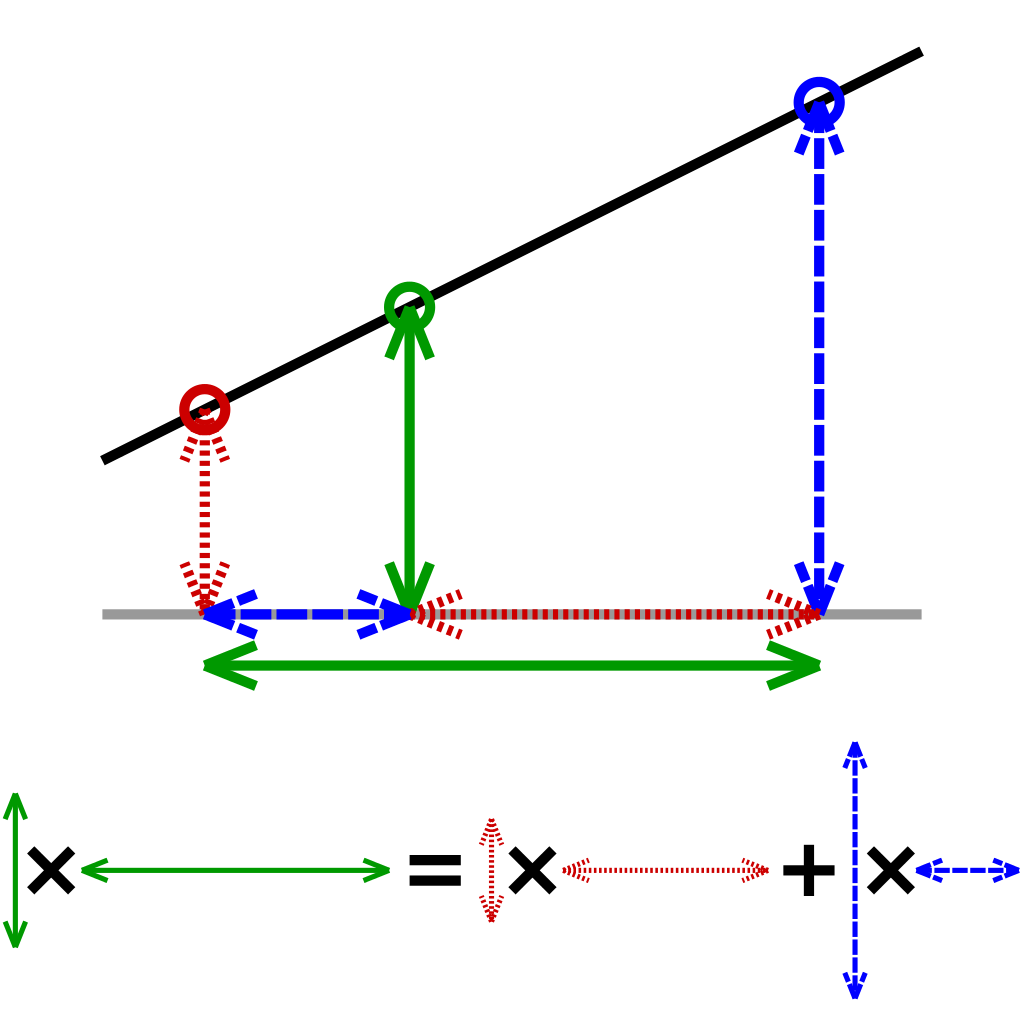
\includegraphics[scale=0.23]{figures/linear_interpolation_visualisation.png}
    \caption{Linear Interpolation Geometric Visualization \cite{Cmglee_linear_interpolation_2022}}
    \label{fig:linear_interpolation_vis}
\end{figure}

Figure \ref{fig:linear_interpolation_vis} shows a geometric representation of linear interpolation. The value at the green circle multiplied by the horizontal distance between the red and blue circles is equal to the sum of the value at the red circle multiplied by the horizontal distance between the green and blue circles, and the value at the blue circle multiplied by the horizontal distance between the green and red circles. \cite{Cmglee_linear_interpolation_2022}

The results of linear interpolation are shown in Table \ref{tab:After_Interpolation}

\begin{table}[H]
\centering
\renewcommand{\arraystretch}{0.75}
\caption{Six Months of U.S. Housing Supply and Price Data with Interpolated Values}
\label{tab:After_Interpolation}
\begin{tabular}{c|c|c} \hline
\textbf{DATE}   & \textbf{MSACSR}     & \textbf{MSPUS}  \\ 
\hline \hline
1963-01-01      & 4.7                 & 17800.00        \\
1963-02-01      & 6.6                 & 17866.67        \\
1963-03-01      & 6.4                 & 17933.33        \\
1963-04-01      & 5.3                 & 18000.00        \\
1963-05-01      & 5.1                 & 17966.67        \\
1963-06-01      & 6.0                 & 17933.33        \\
1963-07-01      & 4.6                 & 17900.00        \\
\hline
\end{tabular}
\end{table}

\subsubsection{Removing Remaining Null Values}

Figure \ref{fig:null_count_by_column} shows the remainder of null values are located mostly in the three columns `10 Year Stock Real Return', `10 Year Bonds Real Return', and `10 Year Excess Returns' with 120 missing values from the years 2012 through 2022 corresponding to the 10 years forward that haven't been `completed.' The remaining missing values consist of 1 each from the `Dividend' and `Real Dividend' columns, as well as 4 from `Earnings', `Real Earnings', and `Real TR Scaled Earnings' respectively.

\begin{figure}[h!]
    \centering
    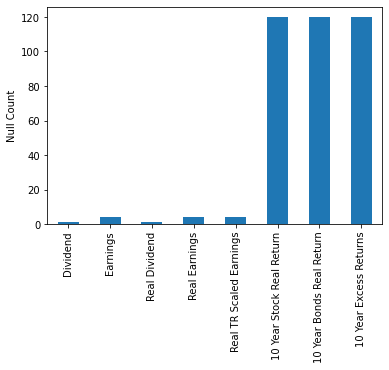
\includegraphics[scale=0.75]{figures/null_count_by_column.png}
    \caption{Missing Values by Column}
    \label{fig:null_count_by_column}
\end{figure}

Because the majority of null values come from only 3 of our 18 features, and there is a possibility of some target variable leakage in these forward-looking values, we remove all 3 of the `10 Year' columns. This leaves only 14 more null values to be managed and maintains all 712 rows of data.

When the remaining null values are plotted by year in which they occur as in Figure \ref{fig:null_count_by_year}, we see that they all are in the tail of the dataset in the year 2022.

\begin{figure}[h!]
    \centering
    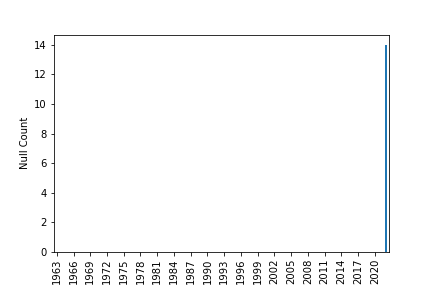
\includegraphics[scale=0.75]{figures/null_count_by_year.png}
    \caption{Missing Values by Year}
    \label{fig:null_count_by_year}
\end{figure}

All 4 null values are in the last 4 months of the dataset, meaning we can remove these rows without creating holes in the middle of the time series and only losing less than 1 percent of the data. This takes the total number of rows from 712 to 708.




\section{Differencing}

Figure \ref{fig:major_variables} shows several features plotted against time. Notice the apparent upward trends in many of the features including CPI, S\&P Composite, and our target variable MSPUS. We apply differencing techniques to reduce this auto-correlation.\cite{Hyndman_stationarity_2021}

\begin{figure}[h!]
    \centering
    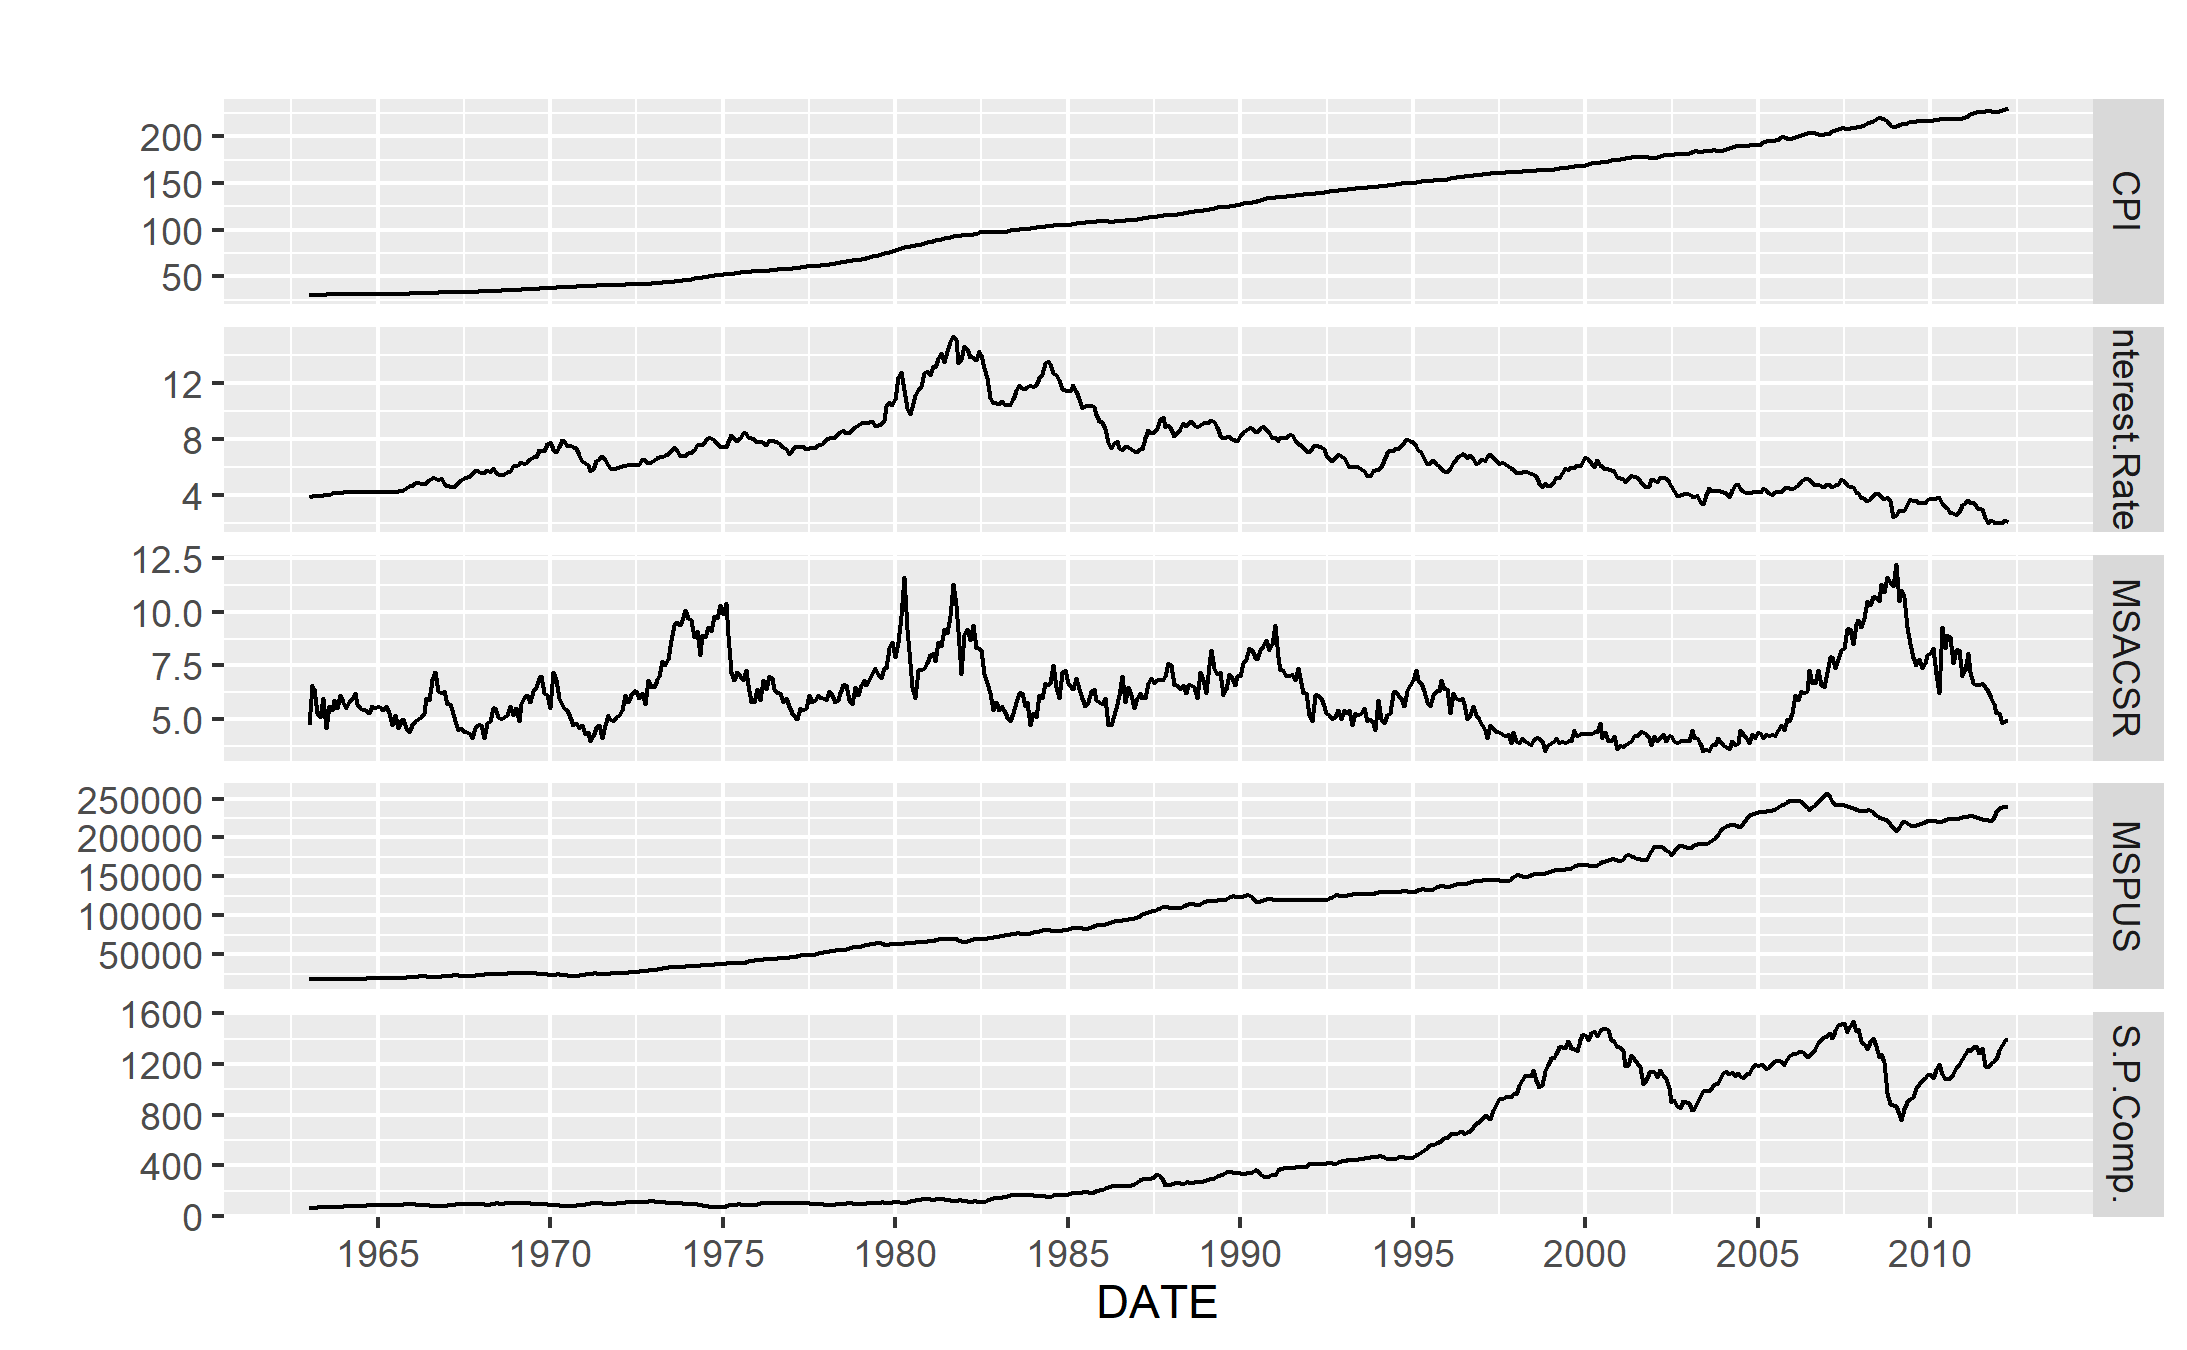
\includegraphics[scale=0.75]{figures/major_variables.png}
    \caption{Select Timeseries Feature Plot}
    \label{fig:major_variables}
\end{figure}


\subsection{First Order Differencing}

A first order price difference calculated by subtracting each value by the previous value in the time series converts the data to a series of changes, one at each time-step $x_t$. 

$$
\begin{aligned}
\hat{x}_{t} &= x_{t} - x_{t-1} \\
\end{aligned}
$$

The result of first order differencing on the median housing price data is shown in Figure \ref{fig:mspus_1st_difference}, where each value represents the month to month change in median home prices. Note the heteroscedasticity, with variance increasing as time progresses. This is due to price swings tending to be larger as housing gets more expensive over time. 

\begin{figure}[h!]
    \centering
    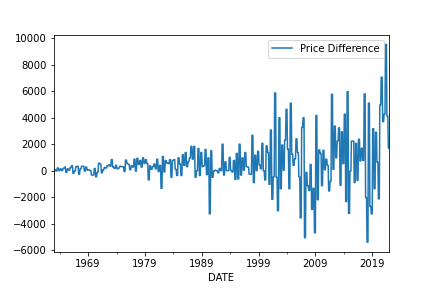
\includegraphics[scale=0.75]{figures/price_1st_difference.png}
    \caption{Monthly First Order Difference of Median U.S. House Prices}
    \label{fig:mspus_1st_difference}
\end{figure}

\subsection{Logarithmic Differencing}

We would like the variance to remain constant over the course of the time series, this is done by instead logarithmic (log) differencing, also known as converting the price data to log returns.

$$
\begin{aligned}
\hat{x}_{t} &= \ln{x_{t}} - \ln{x_{t-1}} \\
\end{aligned}
$$

Where $\hat{x}_{t}$ is the symmetric percent change from $x$ at time $t-1$ to time $t$.


Note that the inverse can be calculated to restore the original data, to reproduce $x_{t}$ from $\hat{x}_{t}$, as long as the first value $x_0$ of the original data vector is known, using the following formula

$$
\begin{aligned}
x_{t} &= {x_{0}} \exp{\sum_{i=1}^{t}{\hat{x}_i}} \\
\end{aligned}
$$
This is used later to transform our log return results into price values.

Figure \ref{fig:logdiff_mspus} shows median housing price data after log differencing. Taking the log has removed the trend same as first order differencing, but also reduced apparent changes in variance and made the data more homoscedastic. An extra benefit of log differencing is that values represent a symmetric percent change where negative and positive values change the direction but not the value of the percent change.\cite{cole_statistics_2017}

\begin{figure}[h!]
    \centering
    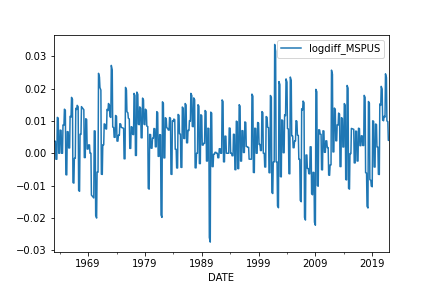
\includegraphics[scale=0.75]{figures/logdiff_MSPUS.png}
    \caption{Log Differencing of Median Housing Prices}
    \label{fig:logdiff_mspus}
\end{figure}

Additionally, as shown in Figure \ref{fig:autocorr}, most of the autocorrelation caused by trending has been reduced. The remaining autocorrelation is only strong in the first 3 or 4 months, with a small amount near the 10 month range. We will use these values when building our LSTM model.

\begin{figure}[h!]
    \centering
    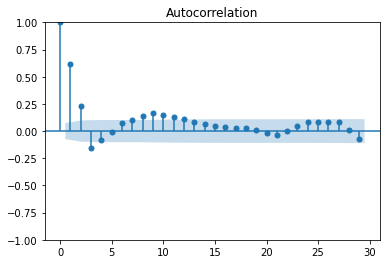
\includegraphics[scale=0.75]{figures/autocorrelation_mspus_tr.png}
    \caption{Autocorrelation of Transformed Housing Prices}
    \label{fig:autocorr}
\end{figure}

\subsection{Application to Data}

WHICH COLUMNS THIS IS APPLIED TO

We apply differencing and log differencing to each feature column depending on which is appropriate


\section{Exploratory Analysis}

DISCUSS TYPE OF CORRELATION USED AND WHY (PEARSON OR KENDALL)

Figure \ref{fig:feature_corr_heatmap} shows a correlation heatmap for all of the features. As one might expect, many of the features that are generally associated with a good economy, such as the S\&P Composite and Earnings, are positively correlated. The Long Interest Rate, which is the yield on 10-year U.S. treasury bonds and is considered the "risk-free rate"\cite{merton_optionpricing_1973}, is negatively correlated with most of the positively correlated STUFF
Interestingly, Monthly Total Bond Returns show almost zero correlation with any other features.

\begin{figure}[h!]
    \centering
    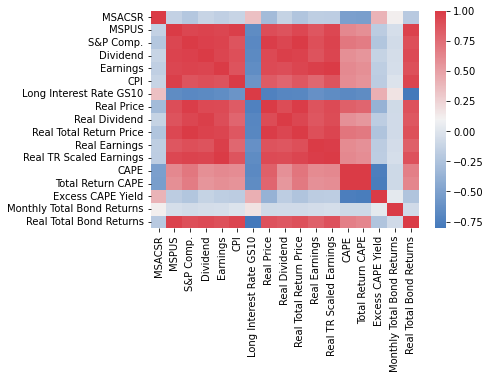
\includegraphics[scale=0.75]{figures/feature_corr_heatmap.png}
    \caption{Correlation Heatmap for All Features}
    \label{fig:feature_corr_heatmap}
\end{figure}


\subsection{Scaling}

Scaling reduces model bias when features have a variety of ranges by normalizing so the model is not dominated by features that have wider ranges. Additionally, gradient descent used by our model converges more quickly with feature scaling than without, allowing for faster training times.\cite{DBLP:journals/corr/IoffeS15}


\subsubsection{Feature Standardization}

Since the ranges of features in the dataset vary, features with a wider range of values may contribute more to the model than those with a narrower range, creating bias. We use scaling to reduce the risk of this happening by standardizing the features to have a mean of zero and standard deviation of one. This is done by applying the following formula to each value $x$ for each feature:

$$
\begin{aligned}
z &= \frac{x - \bar{x}}{\sigma} \\
\end{aligned}
$$

Where $\bar{x}$ is the mean of that feature vector 

$$
\begin{aligned}
\bar{x} &= \frac{1}{n}\sum_{i=1}^{n}{x_i} \\
\end{aligned}
$$

$n$ is the number of values in the feature vector and $\sigma$ is the sample standard deviation

$$
\begin{aligned}
\sigma &= \sqrt{ \frac{1}{n-1}\sum_{i=1}^{n}\left({x_i - \bar{x}}\right)^2}\\
\end{aligned}
$$


\subsubsection{Target Min-Max Normalization}

For the target variable, the monthly percent change in Median U.S. Housing Prices, we apply min-max normalization so that values are in the range $\left[0, 1\right]$ by subtracting the lowest value from all data points and dividing that by the range of the values.

$$
\begin{aligned}
x_{norm} &= \frac{x - x_{min}}{x_{max} - x_{min}}\\
\end{aligned}
$$


\subsection{Example Table}
The frequency table (Table \ref{tab:Funny_Frequency}) 


\begin{table}[H]
\centering
\renewcommand{\arraystretch}{0.75}
\caption{Funny Frequency Table Proportion Percentage more than 0.1\%}
\label{tab:Funny_Frequency}
\begin{tabular}{c|c|c} \hline
\textbf{funny} & \textbf{count} & \textbf{freq \%} \\ \hline \hline
0              & 2,400,963       & 81.8              \\
1              & 324,532         & 11.0              \\
2              & 100,291         & 3.4               \\
 \hline
\end{tabular}
\end{table}








\chapter{Models}







\section{Training, Validation \& Testing Datasets}
The training,

\section{LSTM Model}
The LSTM model 

Figure \ref{fig:lstm_architecture2} shows a block diagram of an LSTM cell. Instead of a unit that simply applies an element-wise nonlinearity to the affine transformation of inputs and recurrent units, LSTM recurrent networks have “LSTM cells” that have an internal recurrence (a self-loop),in addition to the outer recurrence of the RNN. Each cell has the same inputs and outputs as an ordinary recurrent network, but also has more parameters and asystem of gating units that controls the flow of information. The most important component is the state units(t)i, which has a linear self-loop similar to the leaky units described in the previous section. Here, however, the self-loop weight (or the associated time constant) is controlled by a forget gate unit f(t)i(for time step t and cell i), which sets this weight to a value between 0 and 1 via a sigmoid unit:

\begin{figure}[h!]
    \centering
    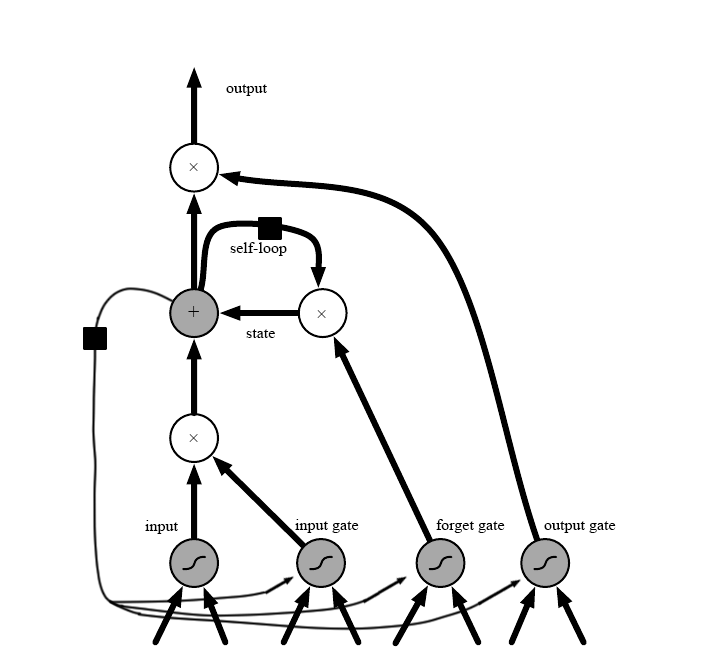
\includegraphics[scale=0.5]{figures/lstm_architecture2.png}
    \caption{Architecture of an LSTM cell\cite{GoodBengCour16}. [REWORD GOODFELLOW p.399] Cells are connected recurrently to each other, replacing the usual hidden units of ordinary recurrent networks.An input feature is computed with a regular artificial neuron unit. Its value can be accumulated into the state if the sigmoidal input gate allows it. The state unit has a linear self-loop whose weight is controlled by the forget gate. The output of the cell can be shut off by the output gate. All the gating units have a sigmoid nonlinearity, while the input unit can have any squashing nonlinearity. The state unit can also be used as an extra input to the gating units. The black square indicates a delay of a single time step}
    \label{fig:lstm_architecture2}
\end{figure}

\subsection{Results}

Figure \ref{fig:actual_vs_pred} shows our predicted values versus the actual median housing prices.

\begin{figure}[h!]
    \centering
    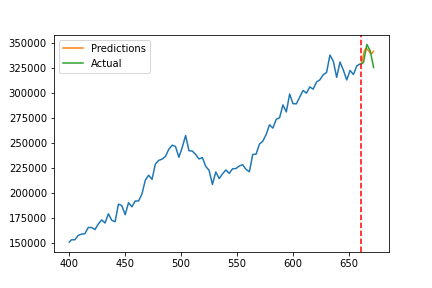
\includegraphics[scale=0.75]{figures/scale_actual_vs_pred.png}
    \caption{Actual vs. Predicted, the predicted slice comes after the dashed red line}
    \label{fig:actual_vs_pred}
\end{figure}

\chapter{Conclusion \& Further Discussion}
\section{Conclusion}
  performance.
 




\section{Further Discussion}
Although 

\nocite{}
\bibliographystyle {uclathes}
\bibliography{myrefs}

\end {document}

